\documentclass[12pt]{article}

\usepackage[spanish]{babel}
\usepackage{hyperref}
\usepackage{graphicx}
\usepackage{listings}
\usepackage{color}
\usepackage{multicol}
\usepackage{amssymb}
\usepackage{enumitem}
\usepackage{here}
\usepackage{dsfont}
\usepackage{amsmath}
\usepackage{tipa}
\usepackage{float}
\spanishdecimal{.}

\title{Matemáticas para las Ciencias Aplicadas I}
\title{
	Tercera Lista de Problemas \\
	\textbf{Segunda  Parte} \\
	\vspace{1ex}
	\large Matemáticas para las Ciencias Aplicadas I \\
	Facultad de Ciencias, UNAM}

\date{\today}

\author{Flores Morán Julieta Melina \\ Zarco Romero José Antonio}

\begin{document}

\maketitle

%% De la sección 4.1: ejercicios 31, 57 y 71.
%% De la sección 4.2: ejercicios 31, 55 y 77.
%% De la sección 4.3: ejercicios 21, 36, 54 y 70.

%% 4.1 -----------------------------------------------------------------------------------------------------------------------------------------------------------------------------------------------------------------------------
\section{Sección 4.1 \\ Análisis De Funciones I: Aumento, Disminución Y Concavidad}
% 31 -------------------------------------------------------------------------------------------------------------
\subsection{Ejercicio 31} name \\

Encuentre: (a) los intervalos en los que $f$ aumenta, (b) los intervalos en los que $f$ disminuye, (c) los intervalos abiertos en los que $f$ es cóncava hacia arriba, (d) los intervalos abiertos en los que $f$ es cóncava hacia abajo, y (e) las coordenadas x de todos los puntos de inflexión.
\[
f(x) = \tan^{-1}(x^2-1)
\]

 Podemos determinar si f(x) crece o decrece en un intervalo según si su derivada es positiva o negativa en ese intervalo. Por esta razón, para determinar (a) y (b) primero necesitamos que derivar f(x).
  \begin{equation*}
  \begin{split}
    f'(x)
    &= \frac{d}{dx}(\tan^{-1}(x^2-1)) \\
    &= \frac{1}{1+(x^{2}-1)^{2}} \cdot \frac{d}{dx}((x^{2}-1)) \\
    &= \frac{1}{1+(x^{2}-1)^{2}} \cdot 2x \\
    \therefore
    f'(x)
    &= \frac{2x}{1+(x^{2}-1)^{2}}
  \end{split}
  \end{equation*}

  La derivada vale $0$ cuando $2x = 0$, es decir, cuando $x=0$. \\
   - Cuando $x>0$, $f'(x)>0$, es decir, es positiva y por lo tanto es creciente. \\
  - Cuando $x<0$, $f'(x)<0$, es decir, es negativa y por lo tanto es decreciente.\\

 \[
 \therefore
 \text{(a):  el intervalos en los que $f$ aumenta es} [0, \infty]
   \]
\[
  \text {(b):  el intervalos en los que $f$ decrece  es}  (-\infty, 0] \\
    \]

    Para responder a los últimos 3 incisos necesitamos información de la segunda derivada. Así que conviene calcularla.
     \begin{equation*}
  \begin{split}
    f''(x)
    &= \frac{d}{dx}( \frac{2x}{ 1+(x^{2}-1)^{2}  } )  \\
    &= \frac{  ( 1+(x^{2}-1)^{2}) \cdot  \frac{d}{dx} (2x) - \left[ 2x \cdot  \frac{d}{dx}   ( 1+(x^{2}-1)^{2})  \right]  }{ (1+(x^{2}-1)^{2} )^{2}  } \\
    &= \frac{  ( 1+(x^{2}-1)^{2}) \cdot  2 - \left[ 2x \cdot  \frac{d}{dx}   [(x^{2}-1)^{2}]  \right]  }{ (1+(x^{2}-1)^{2} )^{2}  } \\
    &= \frac{  2( 1+(x^{2}-1)^{2}) - \left[ 2x \cdot     2(x^{2}-1) \frac{d}{dx} (x^{2}-1)  \right]  }{ (1+(x^{2}-1)^{2} )^{2}  } \\
    &= \frac{  2( 1+(x^{2}-1)^{2}) - \left[ 2x \cdot     2(x^{2}-1) \cdot  2x  \right]  }{ (1+(x^{2}-1)^{2} ^{2}  } \\
    &= \frac{   2+2(x^{2}-1)^{2} - \left[ 8x^{2} \cdot(x^{2}-1)\right]  }{ (1+(x^{2}-1)^{2} )^{2}  } \\
    &= \frac{   2+2(x^{4}-2x^{2}+ 1) - \left[ 8x^{4} - 8x^{2}  \right]  }{ (1+(x^{2}-1)^{2} )^{2}  } \\
    &= \frac{   2+2x^{4}-4x^{2}+ 2 - 8x^{4} + 8x^{2}  }{ (1+(x^{2}-1)^{2} )^{2}  } \\
    &= \frac{-6x^{4} + 4x^{2} +4 }{ (1+(x^{2}-1)^{2} )^{2}  } \\
    \therefore
    f''(x)
    &= -2\frac{3x^{4} - 2x^{2} - 2 }{ (1+(x^{2}-1)^{2} )^{2}  } \\
  \end{split}
     \end{equation*}

     La concavidad depende del signo de $ f''(x)$. Para identificar estos intervalos primero conviene ubicar en que puntos $ f''(x) = 0$ , para reconocer más facilmente $f''(x)<0$ y $f''(x)>0$·

\[ f''(x) = -2\frac{3x^{4} - 2x^{2} - 2 }{ (1+(x^{2}-1)^{2} )^{2}  } = 0  \]
\[ \iff \]
\[ 3x^{4} - 2x^{2} - 2 = 0 \]

Para calcular  $x$ más fácilmente sustituiemos la variable $x^{2}$ por t.

\[ 3t^{2} - 2t - 2 = 0 \]

Y usaremos la fórmula general.

 \begin{equation*}
  \begin{split}
    t
    &=  \frac{2 \pm \sqrt{4-4(3)(-2)} }{2(3)}  \\
    &=  \frac{2 \pm \sqrt{4+24} }{6}  \\
    &=  \frac{2 \pm \sqrt{28} }{6}  \\
    &=  \frac{2 \pm \sqrt{7 \cdot 4} }{6}  \\
    &=  \frac{2 \pm 2 \sqrt{7} }{6}  \\
    &=  \frac{1 \pm \sqrt{7} }{3}  \\
    \therefore
    x^{2}
    &= \pm \sqrt { \frac {1 \pm \sqrt { 7 } } { 3 }  } \\
  \end{split}
 \end{equation*}

Considerando que $1 -  \sqrt{7} \approx -1.64$, $x = \pm \sqrt {\frac{1 - \sqrt{7}}{3}}$ tiene raices imaginarias.\\
Por lo tanto las raíces reales que nos intersane son
  \[
  x = \pm \sqrt {\frac{1 + \sqrt{7} }{3}} 
  \]
Estos son los puntos de inflexión, donde $f(x) = 0$. Así que evaluaremos cada intervalo que nos es de interés,para conocer el signo de $ f''(x) $. Donde es negativa, es concava hacia abajo y donde es positiva es concava hacia arriba.
  
\begin{table}[h]
\centering
\begin{tabular}{|c|c|}
\hline
Intervalo &  Signo de $f''(x)$ & concavidad hacia \\
\hline
$(-\infty, -\sqrt{\frac{1 + \sqrt{7}}{3}})$ & - & abajo\\
\hline
$(-\sqrt{\frac{1 + \sqrt{7}}{3}}, \sqrt{\frac{1 + \sqrt{7}}{3}})$ & + & arriba \\
\hline
$(\sqrt{\frac{1 + \sqrt{7}}{3}}, \infty)$ & - & abajo \\
\hline
\end{tabular}
\end{table}

 \[
 \therefore
 \text{(c):  el intervalos  en los que $f$ es cóncava hacia arriba } (-\sqrt{\frac{1 + \sqrt{7}}{3}}, \sqrt{\frac{1 + \sqrt{7}}{3}})
   \]
\[
  \text {(d):  los  intervalos en los que $f$  es cóncava hacia abajo  son }  (\sqrt{\frac{1 + \sqrt{7}}{3}}, \infty) \text{ y } (-\infty, -\sqrt{\frac{1 + \sqrt{7}}{3}})

    \]
\[
  \text {(e): las cordenadas x de todos los puntos de inflexión son }  x =  \sqrt {\frac{1 + \sqrt{7} }{3}}  \text{ y }  x = - \sqrt {\frac{1 + \sqrt{7} }{3}} 

    \]
% 57 -------------------------------------------------------------------------------------------------------------
\subsection{Ejercicio 57} name \\

\begin{enumerate}[label=(\alph*)]
\item Demuestre que un polinomio cúbico general
  \[
  f(x) = ax^3 + bx^2 + cx + d \qquad (a\neq 0)
  \]
  tiene exactamente un punto de inflexión.

\item Demuestre que si un polinomio cúbico tiene tres intersecciones en el eje x, entonces el punto de inflexión ocurre en el valor promedio de las intersecciones.

\item Utilice el resultado del inciso (b) para encontrar el punto de inflexión del polinomio cúbico $f(x) = x^3-3x^2 + 2x$, y verifique su resultado usando $f''$ para determinar dónde $f$ es cóncava hacia arriba y cóncava hacia abajo.


\end{enumerate}

% 71 -------------------------------------------------------------------------------------------------------------
\subsection{Ejercicio 71} name \\

Suponiendo que $A, k$ y $L$ son constantes positivas, verifique que la gráfica de $y=L/(1+Ae^{-kt})$ tiene un punto de inflexión en $\left( \frac{1}{k}\ln{A},\frac{1}{2}L \right)$. \\
La fórmula dada es la función que describe el crecimiento de curvas lógisticas. Para conocer los puntos de inflexión, necesitamos conocer la segunda derivada con respecto a t. Si multiplicamos ambos lados de la fórmula por $e^{kt}(1+Ae^{-kt})$, obtenemos:
\[
ye^{kt}(1+Ae^{-kt}) = Le^{kt}
\]
\[
ye^{kt}+yAe^{kt}e^{-kt} =Le^{kt}
\]
\[
ye^{kt}+yAe^{kt-kt} = Le^{kt}
\]
\[
ye^{kt}+yAe^{0} = Le^{kt}
\]
\[
ye^{kt}+yA = Le^{kt}
\]
Y usando derivación implícita podemos obtener:
\[
\frac{d}{dt}[y(e^{kt}+A)] = \frac{d}{dt} (Le^{kt})
\]
\[
y \frac{d}{dt}e^{kt} +  (e^{kt}+A)\frac{dy}{dt} = L\frac{d}{dt}(e^{kt})
\]
\[
yke^{kt} +  (e^{kt}+A)\frac{dy}{dt} = Lke^{kt}
\]
\[
  (e^{kt}+A)\frac{dy}{dt} = Lke^{kt} -yke^{kt} 
\]
\[
 \frac{dy}{dt} = \frac{ ke^{kt} (L-y) } {e^{kt}+A}
 \]
 \[
 \frac{dy}{dt} = \frac{ ke^{kt} (L-y) } {Le^{kt}/y} 
 \]
 \[
 \frac{dy}{dt} = \frac{K} {L} y(L-y) 
 \]
 Necesitamos la segunda derivada.
 \[
\frac{d^{2}y}{dt^{2}}} = \frac{dy}{dt} \left[\frac{K} {L} y(L-y)  \right]
  \]
   \[
   \frac{d^{2}y}{dt^{2}}} =\frac{K} {L} \left[  y\frac{d}{dt}(L-y) +(L-yy \frac{dy}{dt}  \right]
     \]
 \[
 \frac{d^{2}y}{dt^{2}}} =\frac{K} {L} \left[  (y)(-\frac{dy}{dt)
     }) +(L-y)  \frac{dy}{dt}  \right]
   \]
  \[
 \frac{d^{2}y}{dt^{2}}} =\frac{K} {L} \left[  (y)(-[\frac{K} {L} y(L-y) ]
     }) +(L-y)  \frac{K} {L} y(L-y)   \right]
     \]
 \[
 \frac{d^{2}y}{dt^{2}}} =\frac{K} {L} \left[ - y^{2}\frac{K} {L}(L-y) 
 +(L-y)^{2}  \frac{K} {L} y   \right]
     \]
%% 4.2 -----------------------------------------------------------------------------------------------------------------------------------------------------------------------------------------------------------------------------
\section{Sección 4.2 \\ Análisis De Funciones II: Extremos Relativos; Graficar Polinomios} 
% 31 -------------------------------------------------------------------------------------------------------------
\subsection{Ejercicio 31} name \\

Utilice la derivada dada para encontrar todos los puntos críticos de $f$ y en cada punto crítico determine si ocurre un máximo relativo, un mínimo relativo o ninguno de los dos. Supongamos en cada caso que $f$ es continua en todas partes.
\[
f'(x)=\ln{\left( \frac{2}{1+x^2} \right)}
\]

% 55 -------------------------------------------------------------------------------------------------------------
\subsection{Ejercicio 55} name \\

Haz una gráfica del polinomio y etiqueta las coordenadas de las intersecciones, los puntos estacionarios y los puntos de inflexión. Comprueba tu trabajo con una utilidad gráfica.
\[
p(x) = (x + 1)^2 (2x-x^2 )
\]
Primero, podemos calcular las intersecciones con los ejes. \\
-Intersecciones con el eje x:
\[
p(x) = (x + 1)^2 (2x-x^2 ) = 0 \iff 
\]
\[
x+1 = 0 \iff  x = -1 \text{ o } 
 \]
 \[
 2x-x^{2}=0 \iff x = 0, 2
 \]
 Por lo que los puntos de intersección con x son:
 \[
(0,0), (2,0), (-1, 0)
 \]
 Donde -1 es un raíz con una multiplicidad de 2, entonces la gráfica de p(x) será tangente al eje x en x=-1, pero no lo cruzara y no habrá un punto de inflexión aquí. 0 y 2 tienen multiplicidad simple, por lo que la grafica no es tangente al eje x en x=0 y x=2, cruza el eje x ahí y puede o no tener un punto de inflexión aquí.\\
 -Intersección con el eje y:\\
 \[
 p(0) = (0 + 1)^2 (2\cdot0-0^2) = 0
 \]
 
 La intersección en ambos ejes se da en (0,0).\\

 Los puntos estacionarios se dan cuando p'(x) = 0.\\
 Para saber esto, necesitamos primero calcular p'(x).\\
 \begin{equation*}
  \begin{split}
    p'(x)
    &=  \frac{d} {dx} \left[ (x + 1)^2 (2x-x^2)\right]  \\
    &=   (x + 1)^2  \frac{d} {dx}(2x-x^2) + (2x-x^2) \frac{d} {dx} (x + 1)^2  \\
    &=   (x + 1)^2 (2-2x) + (2x-x^2)  2(x + 1)  \\
    &=   (x + 1) \left(  (x + 1) (2-2x)  +  2(2x-x^2)  \right) \\
    &=   (x + 1) \left(  2x-2x^{2}+2-2x  +  4x-2x^2  \right) \\
    \therefore
    p'(x)
    &=    (x + 1)\left(  -4x^{2} +4x+2\right) \\ \\
  \end{split}
 \end{equation*}


 \[
  p'(x) =    (x + 1)\left(  -4x^{2} +4x+2\right) = 0
  \]
  \[
  \iff
  \]
   \[
  x + 1  = 0 \iff x =-1
  \]
   \[
 -4x^{2} +4x+2  = 0 \iff x = \frac{1 \pm \sqrt{3} }{2}
 \]
 Evaluando estos puntos:
 \[
  p(\frac{1 + \sqrt{3} }{2}) = \left( \left( \frac{1 + \sqrt{3} }{2}\right) + 1 \right)^2 \left(2\left( \frac{1 + \sqrt{3} }{2} \right)- \left( \frac{1 + \sqrt{3} }{2} \right) ^2 \right) = \frac{9+6\sqrt{3}}{4}
  \]
   \[
  p(\frac{1 - \sqrt{3} }{2}) = \left( \left( \frac{1 - \sqrt{3} }{2}\right) + 1 \right)^2 \left(2\left( \frac{1 - \sqrt{3} }{2} \right)- \left( \frac{1 - \sqrt{3} }{2} \right) ^2 \right) = \frac{9-6\sqrt{3}}{4}
  \]
    Por esto, los puntos estacionarios son:
  \[
(\frac{1 + \sqrt{3} }{2},  \frac{9+6\sqrt{3}}{4} \text{  y  }
(\frac{1 - \sqrt{3} }{2}, \frac{9-6\sqrt{3}}{4} )
  \]

Los puntos de inflexión son los puntos donde la segunda derivada es 0. Para esto necesitamos calcular p''(x).
% 77 -------------------------------------------------------------------------------------------------------------
\subsection{Ejercicio 77} name \\

En cada parte, encuentre $k$ de modo que $f$ tenga un extremo relativo en el punto donde $x = 3$.
\begin{enumerate}[label=(\alph*)]
\item $f(x)=x^2+\frac{k}{x}$
\item $f(x)=\frac{x}{x^2+k}$
\end{enumerate}

%% 4.3 -----------------------------------------------------------------------------------------------------------------------------------------------------------------------------------------------------------------------------
\section{Sección 4.3 \\  Análisis De Funciones III: Funciones Racionales, Cúspides Y Tangentes Verticales}
% 21 -------------------------------------------------------------------------------------------------------------
\subsection{Ejercicio 21} name \\

Dibuja una gráfica de la función racional y etiqueta las coordenadas de los puntos estacionarios y los puntos de inflexión. Muestra las asíntotas horizontales, verticales, oblicuas y curvilíneas y etiquétalas con sus ecuaciones. Etiquete los puntos, si los hay, donde la gráfica cruza una asíntota. Comprueba tu trabajo con una utilidad gráfica.
\[
\frac{(x-2)^3}{x^2}
\]

% 36 -------------------------------------------------------------------------------------------------------------
\subsection{Ejercicio 36} name \\

Dé una gráfica de la función e identifique las ubicaciones de todos los puntos críticos y puntos de inflexión. Comprueba tu trabajo con una utilidad gráfica.
\[
5x^{2/3}+x^{5/3}
\]

% 54 -------------------------------------------------------------------------------------------------------------
\subsection{Ejercicio 54} name \\

Utilizando la regla de L'Hôpital se puede verificar que
\begin{align*}
  \lim_{x \to +\infty} \frac{e^x}{x}=+\infty && \lim_{x \to +\infty} \frac{x}{e^x}=0 && \lim_{x \to -\infty} xe^x=0
\end{align*}
En estos ejercicios: (a) Utilice estos resultados, según sea necesario, para encontrar los límites de $f(x)$ cuando $x\rightarrow +\infty$ y cuando $x\rightarrow -\infty$. (b) Dibuje una gráfica de $f(x)$ e identifique todos los extremos relativos, puntos de inflexión y asíntotas (según corresponda). Comprueba tu trabajo con una utilidad gráfica.
\[
f(x)=x^3e^{x-1}
\]

% 70 -------------------------------------------------------------------------------------------------------------
\subsection{Ejercicio 70} name \\

La figura adjunta muestra una gráfica generada por computadora del polinomio $y = 0.1x^5 (x + 1)^2$ usando una ventana de visualización de $[−2, 1.5] \times [−0.2, 0.2]$. Demuestre que la elección de la escala vertical hizo que la computadora pasara por alto características importantes de la gráfica. Encuentra las características que faltaron y haz tu propio boceto del gráfico que muestra las características que faltan.
\begin{figure}[H]
\centering
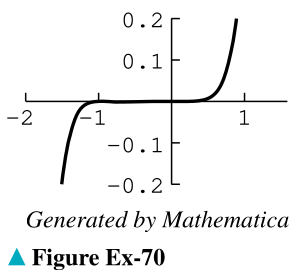
\includegraphics[width=0.4\textwidth]{../img/img_Lista3/2_70.png}
\end{figure}

\end{document}
